%==============================================================
%  EE201 -- Circuit Theory I
%  Lecture 10 : LTI Resistive Circuits and Equivalent One-Ports -- slides
%  M. Mert Ankaralı, METU EEE
%
%  Compile:  ./build.sh      (or: pdflatex EE201_Lecture_10_slides.tex, twice)
%  Same colour code as the handout:
%      charge = purple, current = blue, voltage = orange, power = green
%==============================================================
\documentclass[11pt,aspectratio=169]{beamer}

\usepackage[T1]{fontenc}
\usepackage[utf8]{inputenc}
\usepackage[english]{babel}
\usepackage{lmodern}
\usepackage{amsmath,amssymb}
\usepackage{booktabs}
\usepackage{array}
\usepackage{colortbl}
\usepackage{tikz}
\usepackage[american,siunitx]{circuitikz}
\usetikzlibrary{matrix,arrows.meta,positioning,calc,decorations.pathreplacing,decorations.pathmorphing,decorations.markings}
\usetikzlibrary{overlay-beamer-styles}

%-------------------- plain METU-flavoured theme --------------
\usetheme{default}
\usecolortheme{default}
\useinnertheme{rectangles}
\setbeamertemplate{navigation symbols}{}
\setbeamertemplate{itemize items}[square]
\setbeamerfont{frametitle}{size=\large,series=\bfseries}
\setbeamerfont{title}{size=\LARGE,series=\bfseries}

\definecolor{metured}{RGB}{155,27,48}
\definecolor{metugray}{RGB}{88,89,91}
\definecolor{metulight}{RGB}{243,240,241}
\definecolor{ccur}{RGB}{0,102,170}
\definecolor{cvolt}{RGB}{214,120,0}
\definecolor{cpow}{RGB}{23,128,74}
\definecolor{ccharge}{RGB}{124,60,160}
\definecolor{cflux}{RGB}{0,138,138}
\definecolor{copper}{RGB}{184,98,30}

\setbeamercolor{structure}{fg=metured}
\setbeamercolor{frametitle}{fg=metured,bg=}
\setbeamercolor{title}{fg=metured}
\setbeamercolor{normal text}{fg=black!88}
\setbeamercolor{block title}{fg=white,bg=metured}
\setbeamercolor{block body}{bg=metulight}
\setbeamercolor{alerted text}{fg=metured}

\setbeamertemplate{frametitle}{%
  \vspace{0.55em}%
  \usebeamerfont{frametitle}\usebeamercolor[fg]{frametitle}\insertframetitle\par
  \vspace{-0.2em}{\color{metured}\rule{\textwidth}{1pt}}\par\vspace{-0.2em}}

\setbeamertemplate{footline}{%
  \hbox{\begin{beamercolorbox}[wd=\paperwidth,ht=2.4ex,dp=1.4ex,leftskip=1.2em,rightskip=1.2em]{}%
  \tiny\color{metugray}\coursecode\ \textbar\ Lecture 10: LTI Resistive Circuits and Equivalent One-Ports
  \hfill \insertframenumber/\inserttotalframenumber
  \end{beamercolorbox}}}

%-------------------- macros ----------------------------------
\newcommand{\coursecode}{EE201}
\newcommand{\term}{Fall 2026--2027}
\newcommand{\Icol}[1]{\textcolor{ccur}{#1}}
\newcommand{\Vcol}[1]{\textcolor{cvolt}{#1}}
\newcommand{\Pcol}[1]{\textcolor{cpow}{#1}}
\newcommand{\Qcol}[1]{\textcolor{ccharge}{#1}}
\newcommand{\Fcol}[1]{\textcolor{cflux}{#1}}
\newcommand{\uni}[1]{\,\mathrm{#1}}
\newcommand{\A}{\uni{A}} \newcommand{\V}{\uni{V}}
\newcommand{\W}{\uni{W}} \newcommand{\J}{\uni{J}}
\newcommand{\Cb}{\uni{C}} \newcommand{\s}{\uni{s}}
\newcommand{\Wb}{\uni{Wb}} \newcommand{\Hy}{\uni{H}}
\newcommand{\Sie}{\uni{S}}


\ctikzset{bipoles/length=0.9cm, label/align=straight,
          bipoles/generic/height=0.28, bipoles/generic/width=0.62}
\tikzset{
  iar/.style={-{Stealth[length=2.2mm]}, ccur, thick},
  glab/.style={font=\footnotesize, text=metured},
  ttl/.style={font=\scriptsize\bfseries, text=metugray},
  capn/.style={font=\scriptsize, text=metugray, align=center},
  pol/.style={font=\small, text=cvolt},
  nlab/.style={circle, draw=metured, text=metured, font=\scriptsize, inner sep=0.7pt},
  blab/.style={font=\footnotesize, text=black!80},
  gbr/.style={black!75, thick, postaction={decorate, decoration={markings,
      mark=at position 0.56 with {\arrow{Stealth[length=2.5mm]}}}}},
  hal/.style={draw=cpow!60, line width=6pt, opacity=0.35, line cap=round, line join=round},
  halo/.style={circle, fill=metured!16, minimum size=0.95cm},
  elem/.style={draw=metugray, thick, fill=metulight},
  bigarr/.style={-{Stealth[length=3mm]}, very thick, metugray},
}

%-------------------- Lecture 10 circuit macros ---------------
\newcommand{\ohm}{\,\Omega}
%  Port terminals a (top) and b (bottom) at x = #1, with i (entering at a) and v
\newcommand{\portlabels}[1]{%
  \draw[fill=white] (#1,1.6) circle (1.8pt) node[above=1pt, font=\small] {$a$};
  \draw[fill=white] (#1,0.4) circle (1.8pt) node[below=1pt, font=\small] {$b$};
  \draw[iar] (#1-0.78,1.84) -- (#1-0.22,1.84);
  \node[font=\small, text=ccur] at (#1-0.5,2.12) {$i$};
  \node[pol] at (#1,1.28) {$+$}; \node[pol] at (#1,0.72) {$-$};
  \node[font=\small, text=cvolt] at (#1+0.3,1.0) {$v$};}
%  Two boxes joined at a port: #1 left name, #2 right name
\newcommand{\pairbox}[2]{%
  \draw[elem] (0,0) rectangle (1.7,2.0); \node at (0.85,1.0) {#1};
  \draw[elem] (3.5,0) rectangle (5.2,2.0); \node at (4.35,1.0) {#2};
  \draw (1.7,1.6) -- (3.5,1.6); \draw (1.7,0.4) -- (3.5,0.4);
  \portlabels{2.6}}
%  Substitution: N2 replaced by a voltage source (#1 = 0) or a current source (#1 = 1)
\newcommand{\subsbox}[1]{%
  \draw[elem] (0,0) rectangle (1.7,2.0); \node at (0.85,1.0) {$N_1$};
  \draw (1.7,1.6) -- (3.6,1.6); \draw (1.7,0.4) -- (3.6,0.4);
  \ifcase#1
    \draw (3.6,0.4) to[american voltage source, invert] (3.6,1.6);
    \node[font=\small, right] at (3.95,1.0) {$\Vcol{v_s} = \Vcol{v}$};
  \or
    \draw (3.6,1.6) to[american current source] (3.6,0.4);
    \node[font=\small, right] at (3.95,1.0) {$\Icol{i_s} = \Icol{i}$};
  \fi
  \portlabels{2.6}}
%  A one-port N seen from its terminals
\newcommand{\oneport}[1]{%
  \draw[elem] (1.3,0) rectangle (2.9,2.0); \node at (2.1,1.0) {#1};
  \draw (0,1.6) -- (1.3,1.6); \draw (0,0.4) -- (1.3,0.4);
  \draw[fill=white] (0,1.6) circle (1.8pt) node[left=1pt, font=\small] {$a$};
  \draw[fill=white] (0,0.4) circle (1.8pt) node[left=1pt, font=\small] {$b$};
  \draw[iar] (0.3,1.84) -- (0.95,1.84); \node[font=\small, text=ccur] at (0.62,2.12) {$i$};
  \draw[iar] (0.95,0.16) -- (0.3,0.16); \node[font=\small, text=ccur] at (0.62,-0.13) {$i$};
  \node[pol] at (0.3,1.28) {$+$}; \node[pol] at (0.3,0.72) {$-$};
  \node[font=\small, text=cvolt] at (0.65,1.0) {$v$};}
%  Terminals a, b at (#1,#2) and (#1,0); labels on side #3 (left/right)
\newcommand{\abterm}[3]{%
  \draw[fill=white] (#1,#2) circle (1.8pt) node[#3=1pt, font=\small] {$a$};
  \draw[fill=white] (#1,0) circle (1.8pt) node[#3=1pt, font=\small] {$b$};}
%  k resistors in series between a and b
\newcommand{\seriesR}{%
  \draw (0,1.2) to[R, l=$R_1$] (1.3,1.2) to[R, l=$R_2$] (2.6,1.2) -- (2.8,1.2);
  \node at (3.15,1.2) {$\cdots$};
  \draw (3.5,1.2) -- (3.7,1.2) to[R, l=$R_k$] (5.0,1.2) -- (5.0,0) -- (0,0);
  \abterm{0}{1.2}{left}}
%  k voltage sources in series between a and b (+ towards a)
\newcommand{\seriesV}{%
  \draw (0,1.2) to[american voltage source, l=$v_{s1}$] (1.3,1.2)
        to[american voltage source, l=$v_{s2}$] (2.6,1.2) -- (2.8,1.2);
  \node at (3.15,1.2) {$\cdots$};
  \draw (3.5,1.2) -- (3.7,1.2) to[american voltage source, l=$v_{sk}$] (5.0,1.2)
        -- (5.0,0) -- (0,0);
  \abterm{0}{1.2}{left}}
%  k resistors in parallel between a and b
\newcommand{\parR}{%
  \draw (0,1.5) -- (4.2,1.5); \draw (0,0) -- (4.2,0);
  \draw (0.8,1.5) to[R, l=$R_1$] (0.8,0);
  \draw (2.0,1.5) to[R, l=$R_2$] (2.0,0);
  \node at (3.25,0.75) {$\cdots$};
  \draw (4.2,1.5) to[R, l=$R_k$] (4.2,0);
  \abterm{0}{1.5}{left}}
%  k current sources in parallel between a and b (arrows towards a)
\newcommand{\parI}{%
  \draw (0,1.5) -- (4.2,1.5); \draw (0,0) -- (4.2,0);
  \draw (0.8,0) to[american current source, l_=$i_{s1}$] (0.8,1.5);
  \draw (2.0,0) to[american current source, l_=$i_{s2}$] (2.0,1.5);
  \node at (3.25,0.75) {$\cdots$};
  \draw (4.2,0) to[american current source, l_=$i_{sk}$] (4.2,1.5);
  \abterm{0}{1.5}{left}}
%  One equivalent element between a (height #1) and b; #2: circuitikz options
\newcommand{\eqone}[2]{%
  \draw (0,#1) -- (1.0,#1) to[#2] (1.0,0) -- (0,0);
  \abterm{0}{#1}{left}}
%  Voltage source v_s (#1) in series with R (#2), terminals on the right
\newcommand{\vsR}[2]{%
  \draw (0,0) to[american voltage source, invert, l=#1] (0,1.8);
  \draw (0,1.8) to[R, l=#2] (1.7,1.8) -- (2.4,1.8);
  \draw (0,0) -- (2.4,0);
  \abterm{2.4}{1.8}{right}}
%  Current source i_s (#1) in parallel with R (#2), terminals on the right
\newcommand{\isR}[2]{%
  \draw (0,0) to[american current source, l=#1] (0,1.8);
  \draw (0,1.8) -- (2.4,1.8); \draw (0,0) -- (2.4,0);
  \draw (1.2,1.8) to[R, l=#2] (1.2,0);
  \abterm{2.4}{1.8}{right}}
%  Port current i entering at a and port voltage v, for \vsR / \isR
\newcommand{\stport}{%
  \draw[iar] (2.25,2.07) -- (1.85,2.07); \node[font=\small, text=ccur] at (2.05,2.35) {$i$};
  \node[pol] at (2.45,1.35) {$+$}; \node[pol] at (2.45,0.45) {$-$};
  \node[font=\small, text=cvolt] at (2.75,0.9) {$v$};}
%  The example circuit: 12 V, 2 ohm, 6 ohm in N1; at the port:
%  #1 = 0: 3 ohm, 1: 6 V source, 2: 2 A source
\newcommand{\exN}[1]{%
  \draw[dashed, metugray, rounded corners=3pt] (-0.95,-0.4) rectangle (2.55,2.5);
  \node[font=\small, text=metugray, anchor=south west, inner sep=1pt] at (-0.95,2.52) {$N_1$};
  \draw (0,0) to[american voltage source, invert, l=$12\V$] (0,2);
  \draw (0,2) to[R, l=$2\ohm$] (2.0,2) -- (3.6,2);
  \draw (2.0,2) to[R, l_=$6\ohm$] (2.0,0);
  \draw (0,0) -- (3.6,0);
  \ifcase#1
    \draw (3.6,2) to[R, l=$3\ohm$] (3.6,0);
  \or
    \draw (3.6,0) to[american voltage source, invert, l_=$6\V$] (3.6,2);
  \or
    \draw (3.6,2) to[american current source, l=$2\A$] (3.6,0);
  \fi
  \draw[fill=white] (2.85,2) circle (1.8pt) node[above=1pt, font=\small] {$a$};
  \draw[fill=white] (2.85,0) circle (1.8pt) node[below=1pt, font=\small] {$b$};}
%  Small classification circuits: source #1 and element #2 (circuitikz options)
\newcommand{\mini}[2]{%
  \draw (0,0) to[#1] (0,1.5) -- (1.4,1.5) to[#2] (1.4,0) -- (0,0);}
\newcommand{\yes}{\textcolor{cpow}{\checkmark}}
\newcommand{\no}{\textcolor{metured}{$\boldsymbol{\times}$}}
\newcommand{\U}[2]{\uncover<#1->{#2}}
\hypersetup{colorlinks=true,allcolors=metured}

\title{Lecture 10: LTI Resistive Circuits\\ and Equivalent One-Ports}
\subtitle{EE201 -- Circuit Theory I}
\author{M. Mert Ankaralı}
\institute{\small Department of Electrical and Electronics Engineering\\
           Middle East Technical University}
\date{}

%  Roadmap of the lecture; #1 = current part (1-5)
\newcommand{\rmitem}[3]{%
  \item \ifnum#1<\rmcur\relax \textcolor{black!35}{\textbf{#2} --- #3}
          \ \textcolor{cpow}{\checkmark}%
        \else\ifnum#1=\rmcur\relax \textcolor{metured}{\textbf{#2}} --- #3%
        \else \textbf{#2} --- \textcolor{black!60}{#3}\fi\fi}
\newcommand{\roadmapframe}[1]{%
  \begin{frame}{Roadmap}
    \def\rmcur{#1}%
    \vfill
    \begin{enumerate}\itemsep9pt
      \rmitem{1}{LTI resistive circuits}{what the words mean, and what we gain}
      \rmitem{2}{Substitution theorem}{replace a part of a circuit by a source}
      \rmitem{3}{One-ports and equivalence}{the same $i$--$v$ characteristic at the port}
      \rmitem{4}{Series and parallel}{combine resistors and sources}
      \rmitem{5}{One source and one resistor}{exchange a voltage source and a current source}
    \end{enumerate}
    \vfill
  \end{frame}}
%  Example 10.2 after the source transformation: 6 A || 2 || 6 || 3 ohm
\newcommand{\exT}{%
  \draw (0,0) to[american current source, l=$6\A$] (0,2);
  \draw (0,2) -- (4.0,2); \draw (0,0) -- (4.0,0);
  \draw (1.1,2) to[R, l=$2\ohm$] (1.1,0);
  \draw (2.4,2) to[R, l=$6\ohm$] (2.4,0);
  \draw (4.0,2) to[R, l=$3\ohm$] (4.0,0);
  \draw[fill=white] (3.3,2) circle (1.8pt) node[above=1pt, font=\small] {$a$};
  \draw[fill=white] (3.3,0) circle (1.8pt) node[below=1pt, font=\small] {$b$};}

\begin{document}

%--------------------------------------------------------------
\begin{frame}[plain]
  \titlepage
  \vspace{-1.2em}
  \begin{center}\scriptsize\color{metugray}
    \Icol{$\blacksquare$}~current \quad \Vcol{$\blacksquare$}~voltage \quad
    \textcolor{metugray}{$\blacksquare$}~a part of a circuit (box $N$)
  \end{center}
\end{frame}

%--------------------------------------------------------------
\begin{frame}{Review: equations from the graph alone}
  \vfill
  \begin{center}
  \renewcommand{\arraystretch}{1.35}
  \begin{tabular}{@{}l l l@{}}
  \toprule
   & \textbf{incidence / mesh} & \textbf{fundamental cutset / loop}\\
  \midrule
  KCL & $A\Icol{\mathbf{i}} = \mathbf{0}$ & $Q\Icol{\mathbf{i}} = \mathbf{0}$\\
  KVL & $M\Vcol{\mathbf{v}} = \mathbf{0}$ & $B\Vcol{\mathbf{v}} = \mathbf{0}$\\
  $n - 1$ voltages & node voltages $\Vcol{\mathbf{e}}$ & tree voltages $\Vcol{\mathbf{v}_T}$\\
  $b - n + 1$ currents & mesh currents $\Icol{\mathbf{i}_M}$ & co-tree currents $\Icol{\mathbf{i}_C}$\\
  works for & $M$: planar, nonseparable & any connected graph\\
  \bottomrule
  \end{tabular}
  \end{center}
  \vfill
  \begin{center}
    KCL and KVL depend only on the graph: they hold for \alert{any} elements.\\[4pt]
    A circuit has $2b$ unknowns: $b$ more equations come from the elements.
  \end{center}
  \vfill
\end{frame}

%--------------------------------------------------------------
\begin{frame}{Why this lecture?}
  \vfill
  \begin{itemize}\itemsep10pt
    \item \textbf{So far:} KCL and KVL, written for \alert{any} elements.
    \item<2-> \textbf{Now:} we restrict the elements. In an \alert{LTI resistive circuit}
      every equation is \alert{linear} and \alert{algebraic}.
    \item<3-> \textbf{Before solving:} simplify. Replace a part of the circuit by a source,
      or by a simpler part with the same behaviour at its terminals.
    \item<4-> \textbf{Tools:} the substitution theorem, equivalent one-ports, series and
      parallel connections, source transformation.
    \item<5-> \textbf{Next:} systematic methods for every LTI resistive circuit
      --- node voltage and mesh current analysis.
  \end{itemize}
  \vfill
\end{frame}

%==============================================================
\roadmapframe{1}

%--------------------------------------------------------------
\begin{frame}{Three pairs of words}
  \vfill
  \begin{center}
  \renewcommand{\arraystretch}{1.5}
  \begin{tabular}{@{}l l l@{}}
  \toprule
  the circuit is \dots & if it contains \dots & otherwise it is \dots\\
  \midrule
  \alert{nonlinear}    & a nonlinear $R$, $L$, $C$ or dependent source & \textbf{linear}\\
  \onslide<2->{\alert{time-varying} & a time-varying $R$, $L$, $C$ or dependent source & \textbf{time-invariant}}\\
  \onslide<3->{\alert{dynamic}      & an $L$ or a $C$ & \textbf{resistive}}\\
  \bottomrule
  \end{tabular}
  \end{center}
  \vfill
  \onslide<4->{%
  \begin{block}{LTI resistive circuit}
    Linear, time-invariant and resistive: it contains only \alert{LTI resistors},
    \alert{linear time-invariant dependent sources} and \alert{independent sources}.
  \end{block}}
  \vfill
\end{frame}

%--------------------------------------------------------------
\begin{frame}{Independent sources do not count}
  \begin{columns}[c,onlytextwidth]
    \begin{column}{0.4\textwidth}
      \centering
      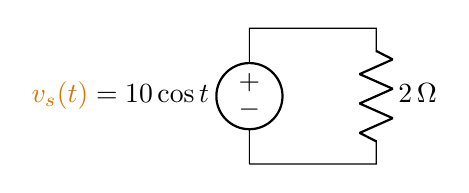
\begin{tikzpicture}[scale=1.15]
        \mini{american voltage source, invert, l={$\Vcol{v_s(t)} = 10\cos t$}}{R, l=$2\ohm$}
      \end{tikzpicture}
    \end{column}
    \begin{column}{0.58\textwidth}
      The source varies in time. Is the circuit time-varying?\\[10pt]
      \onslide<2->{\alert{No.} The three pairs of words look only at $R$, $L$, $C$ and
        \alert{dependent} sources. This is an \alert{LTI resistive} circuit.\\[10pt]}
      \onslide<3->{The words describe the circuit, not the waveform that drives it.}
    \end{column}
  \end{columns}
\end{frame}

%--------------------------------------------------------------
\begin{frame}{Which circuit is which?}
  \vfill
  \begin{center}
  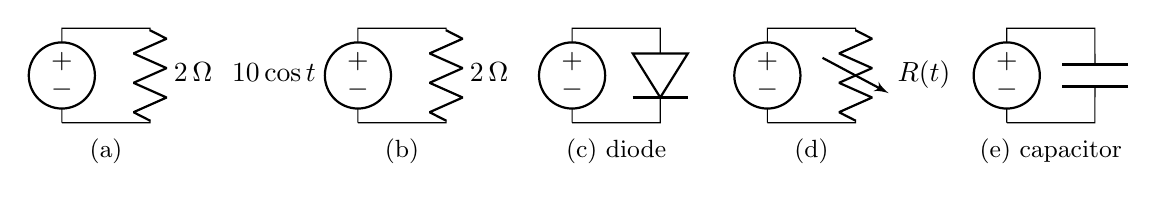
\begin{tikzpicture}[scale=0.8]
    \begin{scope}[shift={(0,0)}]\mini{american voltage source, invert}{R, l=$2\ohm$}
      \node[font=\small] at (0.7,-0.45) {(a)};\end{scope}
    \begin{scope}[shift={(4.7,0)}]\mini{american voltage source, invert, l=$10\cos t$}{R, l=$2\ohm$}
      \node[font=\small] at (0.7,-0.45) {(b)};\end{scope}
    \begin{scope}[shift={(8.1,0)}]\mini{american voltage source, invert}{D}
      \node[font=\small] at (0.7,-0.45) {(c) diode};\end{scope}
    \begin{scope}[shift={(11.2,0)}]\mini{american voltage source, invert}{vR, l=$R(t)$}
      \node[font=\small] at (0.7,-0.45) {(d)};\end{scope}
    \begin{scope}[shift={(15.0,0)}]\mini{american voltage source, invert}{C}
      \node[font=\small] at (0.7,-0.45) {(e) capacitor};\end{scope}
  \end{tikzpicture}
  \end{center}
  \vfill
  \begin{center}
  \only<1>{Sources: $5\V$ except (b). In (d), $R(t) = 2 + \sin t\ \Omega$.\\[4pt] Linear? \quad Time-invariant? \quad Resistive?}%
  \only<2->{%
  \renewcommand{\arraystretch}{1.2}
  \begin{tabular}{@{}l c c c c c@{}}
  \toprule
   & (a) & (b) & (c) & (d) & (e)\\
  \midrule
  linear         & \yes & \yes & \no  & \yes & \yes\\
  time-invariant & \yes & \yes & \yes & \no  & \yes\\
  resistive      & \yes & \yes & \yes & \yes & \no\\
  \midrule
  LTI resistive  & \yes & \yes & \no & \no & \no\\
  \bottomrule
  \end{tabular}}
  \end{center}
  \vfill
\end{frame}

%--------------------------------------------------------------
\begin{frame}{What we gain}
  \vfill
  \begin{itemize}\itemsep10pt
    \item KCL and KVL are \alert{linear}.
    \item<2-> Every element equation is \alert{linear} and \alert{algebraic}:
      \[
        \Vcol{v} = R\Icol{i} \ \ \text{(resistor)}, \qquad
        \Vcol{v} = \mu\Vcol{v_x}, \ \ \Icol{i} = g\Vcol{v_x}, \ \dots \ \
        \text{(dependent sources)}
      \]
      No derivative appears.
    \item<3-> Time enters only through the values of the \alert{independent sources}.
    \item<4-> So at each instant the circuit is solved like a circuit with
      \alert{constant} sources: $2b$ linear algebraic equations.
  \end{itemize}
  \vfill
\end{frame}

%==============================================================
\roadmapframe{2}

%--------------------------------------------------------------
\begin{frame}{The substitution theorem}
  \vfill
  \begin{center}
  \begin{tabular}{@{}c@{\hspace{4mm}}c@{\hspace{4mm}}c@{}}
  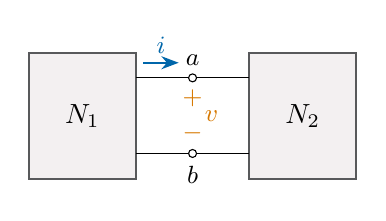
\begin{tikzpicture}[scale=0.8]
    \pairbox{$N_1$}{$N_2$}
  \end{tikzpicture} &
  \onslide<2->{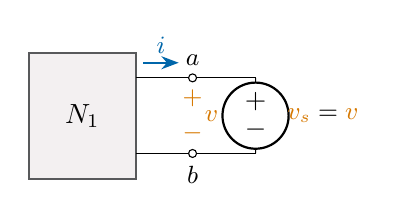
\begin{tikzpicture}[scale=0.8]
    \subsbox{0}
  \end{tikzpicture}} &
  \onslide<3->{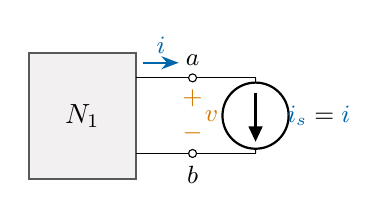
\begin{tikzpicture}[scale=0.8]
    \subsbox{1}
  \end{tikzpicture}}\\[2pt]
  (I) & \onslide<2->{(II)} & \onslide<3->{(III)}
  \end{tabular}
  \end{center}
  \vfill
  \only<1>{\begin{center}A circuit cut into two parts, joined at the terminals $a$, $b$.\\
    $\Icol{i}$: current from $N_1$ into $N_2$ \quad $\Vcol{v}$: voltage between $a$ and $b$
  \end{center}}%
  \only<2>{\begin{center}Replace $N_2$ by a voltage source with $\Vcol{v_s(t)} = \Vcol{v(t)}$
    \dots\end{center}}%
  \only<3>{\begin{center}\dots\ or by a current source with $\Icol{i_s(t)} = \Icol{i(t)}$.
    \end{center}}%
  \only<4->{%
  \begin{block}{Substitution theorem}
    No branch voltage or branch current inside $N_1$ changes. An observer inside $N_1$
    \alert{cannot tell} (I), (II) and (III) apart.
  \end{block}}
  \vfill
\end{frame}

%--------------------------------------------------------------
\begin{frame}{Why does it work?}
  \vfill
  \begin{itemize}\itemsep10pt
    \item The equations inside $N_1$ (KCL, KVL, element equations) do \alert{not} change.
    \item<2-> $N_1$ meets the rest only through $\Vcol{v}$ and $\Icol{i}$.
    \item<3-> The source fixes one of them at the value it had in (I). The solution of (I)
      still satisfies every equation of (II) and (III).
    \item<4-> $N_2$ can be \alert{anything}, even nonlinear: only its port values matter.
  \end{itemize}
  \vfill
  \onslide<5->{%
  \begin{block}{One condition}
    The new circuit must have a \alert{unique} solution. If $N_1$ is a single current source,
    replacing $N_2$ by a current source leaves $\Vcol{v}$ undetermined.
  \end{block}}
  \vfill
\end{frame}

%--------------------------------------------------------------
\begin{frame}{Example: substitution}
  \begin{columns}[c,onlytextwidth]
    \begin{column}{0.46\textwidth}
      \centering
      \begin{tikzpicture}[scale=1.0]
        \only<1-2>{\exN{0}}%
        \only<3>{\exN{1}}%
        \only<4>{\exN{2}}%
        \only<2->{%
          \draw[iar] (0.6,1.72) -- (1.3,1.72);
          \node[font=\small, text=ccur] at (0.95,1.45) {$3\A$};
          \draw[iar] (1.45,0.85) -- (1.45,0.3);
          \node[font=\small, text=ccur, left] at (1.38,0.55) {$1\A$};
          \node[pol] at (2.85,1.6) {$+$}; \node[pol] at (2.85,0.4) {$-$};
          \node[font=\small, text=cvolt] at (2.85,1.0) {$6\V$};
          \draw[iar] (3.05,2.25) -- (3.5,2.25);
          \node[font=\small, text=ccur] at (3.3,2.55) {$2\A$};}
      \end{tikzpicture}
    \end{column}
    \begin{column}{0.52\textwidth}
      \only<1>{$N_2$ is the $3\ohm$ resistor. Find $\Vcol{v}$, $\Icol{i}$ and the currents
        inside $N_1$.}%
      \only<2->{\textbf{(I)} $6\ohm \parallel 3\ohm = 2\ohm$; the two $2\ohm$ share
        $12\V$:\\[3pt]
        \quad $\Vcol{v} = 6\V$, \ $\Icol{i} = 6/3 = 2\A$\\[3pt]
        Inside $N_1$: $\Icol{3\A}$ in the $2\ohm$, $\Icol{1\A}$ in the $6\ohm$.\\[10pt]}%
      \only<3->{\textbf{(II)} A $6\V$ source fixes $\Vcol{v} = 6\V$: again $\Icol{3\A}$ and
        $\Icol{1\A}$. \yes\\[10pt]}%
      \only<4->{\textbf{(III)} A $2\A$ source: KCL at $a$,
        $\tfrac{12 - \Vcol{v}}{2} = \tfrac{\Vcol{v}}{6} + 2$, so $\Vcol{v} = 6\V$:
        again $\Icol{3\A}$ and $\Icol{1\A}$. \yes}
    \end{column}
  \end{columns}
\end{frame}

%==============================================================
\roadmapframe{3}

%--------------------------------------------------------------
\begin{frame}{Ports and one-ports}
  \begin{block}{Port, one-port}
    A pair of terminals is a \alert{port} if the current entering one terminal equals the
    current leaving the other. A \alert{one-port} is a circuit, or a circuit element, with one
    pair of terminals accessible from outside.
  \end{block}
  \vfill
  \begin{columns}[c,onlytextwidth]
    \begin{column}{0.36\textwidth}
      \centering
      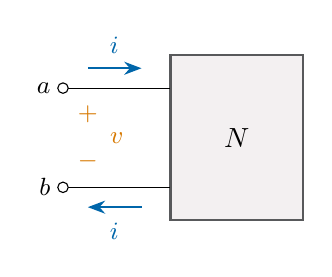
\begin{tikzpicture}[scale=1.05]
        \oneport{$N$}
      \end{tikzpicture}
    \end{column}
    \begin{column}{0.62\textwidth}
      \begin{itemize}\itemsep8pt
        \item<2-> A one-port is always a port: KCL on a closed surface around $N$.
        \item<3-> $\Icol{i}$ enters the $+$ terminal of $\Vcol{v}$.
        \item<4-> The relation between $\Vcol{v}$ and $\Icol{i}$: the
          \alert{$i$--$v$ characteristic}. A resistor: $\Vcol{v} = R\Icol{i}$.
      \end{itemize}
    \end{column}
  \end{columns}
  \vfill
\end{frame}

%--------------------------------------------------------------
\begin{frame}{Equivalent one-ports}
  \begin{block}{Equivalent one-ports}
    $N_1 \equiv N_2$ if they have the \alert{same $i$--$v$ characteristic} at their
    terminals.
  \end{block}
  \vfill
  \begin{center}
  \begin{tabular}{@{}c@{\hspace{12mm}}c@{}}
  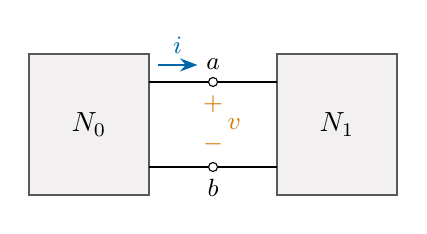
\begin{tikzpicture}[scale=0.9]
    \pairbox{$N_0$}{$N_1$}
  \end{tikzpicture} &
  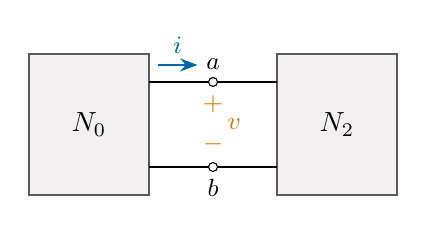
\begin{tikzpicture}[scale=0.9]
    \pairbox{$N_0$}{$N_2$}
  \end{tikzpicture}
  \end{tabular}
  \end{center}
  \vfill
  \begin{center}
    \onslide<2->{For any $N_0$: every branch voltage and current inside $N_0$ is the
      \alert{same} in both.\\[4pt]}
    \onslide<3->{Why: the equations are those of $N_0$ plus the $i$--$v$ characteristic at the
      port.\\[4pt]}
    \onslide<4->{Inside $N_1$ and $N_2$ the branch values \alert{may differ}.}
  \end{center}
  \vfill
\end{frame}

%==============================================================
\roadmapframe{4}

%--------------------------------------------------------------
\begin{frame}{Series connection}
  \centering
  Same current $\Icol{i}$ through every element (KCL); the voltages add (KVL).\\[8pt]
  \begin{tabular}{@{}c@{\hspace{3mm}}c@{\hspace{3mm}}c@{\hspace{6mm}}l@{}}
  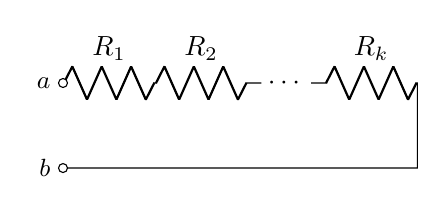
\begin{tikzpicture}[scale=0.9, baseline=(c.base)]
    \seriesR \coordinate (c) at (0,0.5);
  \end{tikzpicture} & $\equiv$ &
  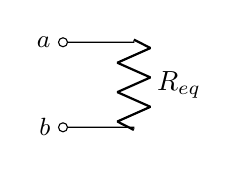
\begin{tikzpicture}[scale=0.9, baseline=(c.base)]
    \eqone{1.2}{R, l=$R_{eq}$} \coordinate (c) at (0,0.5);
  \end{tikzpicture} &
  \onslide<2->{$R_{eq} = R_1 + R_2 + \dots + R_k$}\\[14pt]
  \onslide<4->{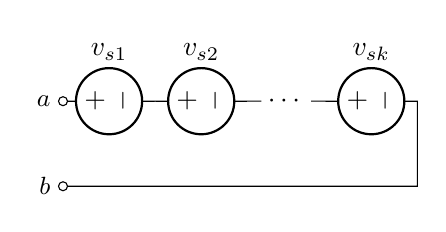
\begin{tikzpicture}[scale=0.9, baseline=(c.base)]
    \seriesV \coordinate (c) at (0,0.5);
  \end{tikzpicture}} & \onslide<4->{$\equiv$} &
  \onslide<4->{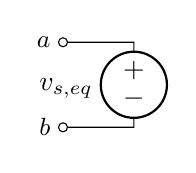
\begin{tikzpicture}[scale=0.9, baseline=(c.base)]
    \eqone{1.2}{american voltage source, l_=$v_{s,eq}$} \coordinate (c) at (0,0.5);
  \end{tikzpicture}} &
  \onslide<4->{$v_{s,eq} = v_{s1} + v_{s2} + \dots + v_{sk}$}
  \end{tabular}\\[10pt]
  \only<2>{$\Vcol{v} = R_1\Icol{i} + R_2\Icol{i} + \dots + R_k\Icol{i} = R_{eq}\Icol{i}$}%
  \only<3>{Voltage divider: the share of $R_j$ is $\Vcol{v_j} = \dfrac{R_j}{R_{eq}}\,\Vcol{v}$}%
  \only<4>{All $+$ signs towards $a$; a source turned the other way enters with $-$.}
\end{frame}

%--------------------------------------------------------------
\begin{frame}{Parallel connection}
  \centering
  Same voltage $\Vcol{v}$ across every element (KVL); the currents add (KCL).\\[8pt]
  \begin{tabular}{@{}c@{\hspace{3mm}}c@{\hspace{3mm}}c@{\hspace{6mm}}l@{}}
  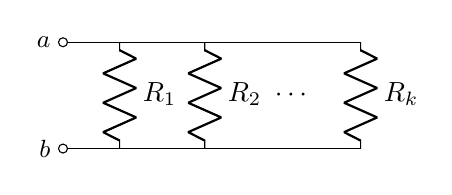
\begin{tikzpicture}[scale=0.9, baseline=(c.base)]
    \parR \coordinate (c) at (0,0.65);
  \end{tikzpicture} & $\equiv$ &
  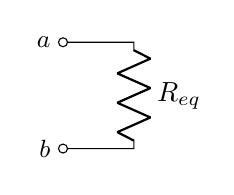
\begin{tikzpicture}[scale=0.9, baseline=(c.base)]
    \eqone{1.5}{R, l=$R_{eq}$} \coordinate (c) at (0,0.65);
  \end{tikzpicture} &
  \onslide<2->{$\dfrac{1}{R_{eq}} = \dfrac{1}{R_1} + \dfrac{1}{R_2} + \dots + \dfrac{1}{R_k}$}\\[14pt]
  \onslide<4->{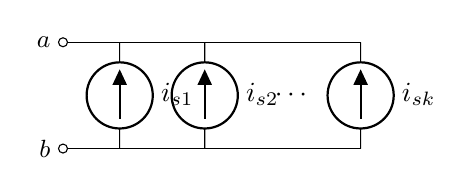
\begin{tikzpicture}[scale=0.9, baseline=(c.base)]
    \parI \coordinate (c) at (0,0.65);
  \end{tikzpicture}} & \onslide<4->{$\equiv$} &
  \onslide<4->{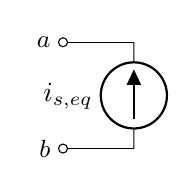
\begin{tikzpicture}[scale=0.9, baseline=(c.base)]
    \draw (1.0,0) to[american current source, l=$i_{s,eq}$] (1.0,1.5);
    \draw (0,1.5) -- (1.0,1.5); \draw (0,0) -- (1.0,0); \abterm{0}{1.5}{left}
    \coordinate (c) at (0,0.65);
  \end{tikzpicture}} &
  \onslide<4->{$i_{s,eq} = i_{s1} + i_{s2} + \dots + i_{sk}$}
  \end{tabular}\\[10pt]
  \only<2>{With $G_j = 1/R_j$: \ $\Icol{i} = G_1\Vcol{v} + \dots + G_k\Vcol{v} =
    G_{eq}\Vcol{v}$, \ $G_{eq} = G_1 + \dots + G_k$}%
  \only<3>{Current divider: $\Icol{i_j} = \dfrac{G_j}{G_{eq}}\,\Icol{i}$. \quad Two
    resistors: $R_{eq} = \dfrac{R_1R_2}{R_1 + R_2}$}%
  \only<4>{All arrows towards $a$; a source turned the other way enters with $-$.}
\end{frame}

%--------------------------------------------------------------
\begin{frame}{Two connections to avoid}
  \begin{columns}[c,onlytextwidth]
    \begin{column}{0.5\textwidth}
      \centering
      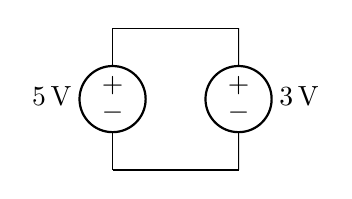
\begin{tikzpicture}[scale=1.0]
        \draw (0,0) to[american voltage source, invert, l=$5\V$] (0,1.8);
        \draw (0,1.8) -- (1.6,1.8); \draw (0,0) -- (1.6,0);
        \draw (1.6,0) to[american voltage source, invert, l_=$3\V$] (1.6,1.8);
      \end{tikzpicture}\\[4pt]
      two voltage sources in parallel\\[10pt]
      \onslide<2->{\alert{KVL fails}: $5 \ne 3$.}
    \end{column}
    \begin{column}{0.5\textwidth}
      \centering
      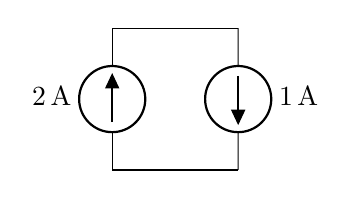
\begin{tikzpicture}[scale=1.0]
        \draw (0,0) to[american current source, l=$2\A$] (0,1.8);
        \draw (0,1.8) -- (1.6,1.8);
        \draw (1.6,1.8) to[american current source, l=$1\A$] (1.6,0);
        \draw (1.6,0) -- (0,0);
      \end{tikzpicture}\\[4pt]
      two current sources in series\\[10pt]
      \onslide<2->{\alert{KCL fails}: $2 \ne 1$.}
    \end{column}
  \end{columns}
  \vfill
  \begin{center}
    \only<1>{Are these allowed?}%
    \only<2->{With \alert{equal} values they are allowed, but the shared current (or voltage)
      is not fixed.}
  \end{center}
\end{frame}

%==============================================================
\roadmapframe{5}

%--------------------------------------------------------------
\begin{frame}{One source and one resistor}
  \vfill
  \begin{center}
  \begin{tabular}{@{}c@{\hspace{18mm}}c@{}}
  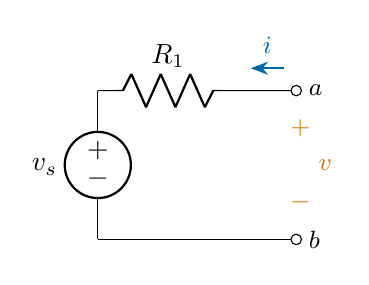
\begin{tikzpicture}[scale=1.05]
    \vsR{$v_s$}{$R_1$} \stport
  \end{tikzpicture} &
  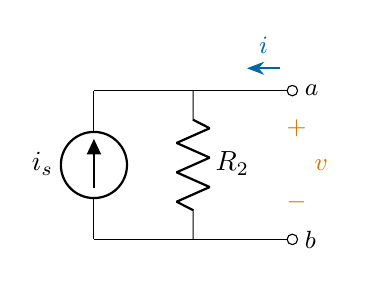
\begin{tikzpicture}[scale=1.05]
    \isR{$i_s$}{$R_2$} \stport
  \end{tikzpicture}\\[6pt]
  \onslide<2->{$\Vcol{v} = R_1\Icol{i} + v_s$} &
  \onslide<3->{$\Vcol{v} = R_2(\Icol{i} + i_s) = R_2\Icol{i} + R_2 i_s$}
  \end{tabular}
  \end{center}
  \vfill
  \begin{center}
    \only<1>{When do these two one-ports have the same $i$--$v$ characteristic?}%
    \only<2>{KVL around the loop: $R_1$ carries $\Icol{i}$.}%
    \only<3>{$\Icol{i}$ and $i_s$ both flow into the top node: $R_2$ carries
      $\Icol{i} + i_s$.}%
    \only<4->{Both are straight lines in the $i$--$v$ plane: equal \alert{slopes} and equal
      \alert{intercepts}.}
  \end{center}
  \vfill
\end{frame}

%--------------------------------------------------------------
\begin{frame}{Source transformation}
  \begin{columns}[c,onlytextwidth]
    \begin{column}{0.5\textwidth}
      \begin{block}{Source transformation}
        The two one-ports are equivalent if
        \[
          R_1 = R_2 = R \qquad\text{and}\qquad v_s = R\, i_s .
        \]
      \end{block}
      \vspace{8pt}
      \onslide<2->{Open circuit ($\Icol{i} = 0$): $\Vcol{v} = v_s$.\\[4pt]}
      \onslide<3->{Short circuit ($\Vcol{v} = 0$): $\Icol{i} = -i_s$.}
    \end{column}
    \begin{column}{0.46\textwidth}
      \centering
      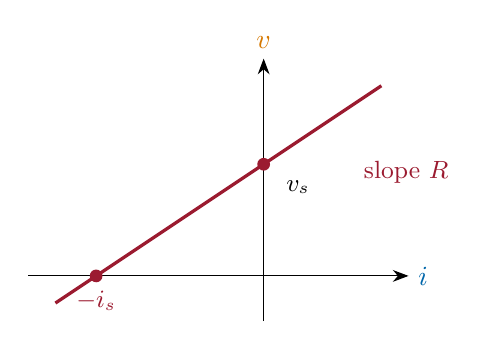
\begin{tikzpicture}[scale=1.15]
        \draw[-{Stealth[length=2mm]}] (-2.6,0) -- (1.6,0) node[right] {$\Icol{i}$};
        \draw[-{Stealth[length=2mm]}] (0,-0.5) -- (0,2.4) node[above] {$\Vcol{v}$};
        \draw[metured, very thick] (-2.3,-0.3) -- (1.3,2.1);
        \node[font=\small, text=metured, anchor=west] at (1.0,1.15) {slope $R$};
        \onslide<2->{\fill[metured] (0,1.233) circle (2pt);
          \node[font=\small] at (0.38,0.98) {$v_s$};}
        \onslide<3->{\fill[metured] (-1.85,0) circle (2pt)
          node[below=2pt, font=\small] {$-i_s$};}
      \end{tikzpicture}
    \end{column}
  \end{columns}
\end{frame}

%--------------------------------------------------------------
\begin{frame}{Example: a source transformation}
  \vfill
  \begin{center}
  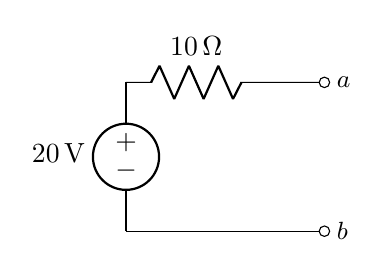
\begin{tikzpicture}[scale=1.05, baseline=(c.base)]
    \vsR{$20\V$}{$10\ohm$} \coordinate (c) at (0,0.8);
  \end{tikzpicture}
  \qquad $\equiv$ \qquad
  \begin{tikzpicture}[scale=1.05, baseline=(c.base)]
    \only<1>{\isR{$?$}{$?$}}%
    \only<2->{\isR{$2\A$}{$10\ohm$}}
    \coordinate (c) at (0,0.8);
  \end{tikzpicture}
  \end{center}
  \vfill
  \begin{center}
    \only<1>{Find the current source and the resistor.}%
    \only<2->{$R = 10\ohm$, \quad $i_s = v_s/R = 20/10 = 2\A$\\[6pt]
      Both: open-circuit voltage $20\V$, short-circuit current $2\A$ (out of $a$).}
  \end{center}
  \vfill
\end{frame}

%--------------------------------------------------------------
\begin{frame}{Example: the substitution example, by transformations}
  \begin{columns}[c,onlytextwidth]
    \begin{column}{0.46\textwidth}
      \centering
      \begin{tikzpicture}[scale=1.0]
        \only<1>{\exN{0}}%
        \only<2>{\exT}%
        \only<3->{%
          \draw (0,0) to[american current source, l=$6\A$] (0,2);
          \draw (0,2) -- (1.6,2); \draw (0,0) -- (1.6,0);
          \draw (1.6,2) to[R, l=$1\ohm$] (1.6,0);
          \node[pol] at (2.6,1.55) {$+$}; \node[pol] at (2.6,0.45) {$-$};
          \node[font=\small, text=cvolt] at (2.6,1.0) {$\Vcol{v}$};}
      \end{tikzpicture}
    \end{column}
    \begin{column}{0.52\textwidth}
      \only<1>{Find $\Vcol{v}$ again, with source transformations only.}%
      \only<2->{$12\V$ with $2\ohm$ in series $\to$ $6\A$ with $2\ohm$ in parallel.\\[8pt]}%
      \only<3->{$2\ohm$, $6\ohm$, $3\ohm$ in parallel:
        $G_{eq} = \tfrac12 + \tfrac16 + \tfrac13 = 1\Sie$, so $R_{eq} = 1\ohm$.\\[6pt]
        $\Vcol{v} = 6\A \times 1\ohm = 6\V$, \quad $\Icol{i} = 6/3 = 2\A$. \yes\\[8pt]}%
      \only<4->{\alert{Careful:} inside the transformed one-port the values differ. The
        $12\V$ source carries $3\A$, the $6\A$ source carries $6\A$.}
    \end{column}
  \end{columns}
\end{frame}

%--------------------------------------------------------------
\begin{frame}{Solving LTI resistive circuits}
  \vfill
  \begin{itemize}\itemsep10pt
    \item Series and parallel connections and source transformations simplify
      \alert{many} circuits, but not all.
    \item<2-> Two systematic methods solve \alert{every} LTI resistive circuit:
      \begin{enumerate}\itemsep4pt
        \item \alert{node voltage analysis}: the $n - 1$ node voltages are the unknowns;
        \item \alert{mesh current analysis}: the $b - n + 1$ mesh currents are the unknowns.
      \end{enumerate}
    \item<3-> Both start from the matrices met earlier ($A$, $M$); now the element
      equations are linear too.
  \end{itemize}
  \vfill
\end{frame}

%--------------------------------------------------------------
\begin{frame}{Summary}
  \vfill
  \begin{itemize}\itemsep7pt
    \item \alert{LTI resistive}: no nonlinear element, no time-varying element, no $L$ or
      $C$. Independent sources do not count. All equations are linear and algebraic.
    \item \alert{Substitution}: replace $N_2$ by a voltage source $\Vcol{v_s} = \Vcol{v}$ or a
      current source $\Icol{i_s} = \Icol{i}$; nothing changes inside $N_1$.
    \item \alert{Equivalent one-ports}: the same $i$--$v$ characteristic; the rest cannot
      tell them apart.
    \item Series: $R_{eq} = \sum R_j$, $v_{s,eq} = \sum v_{sj}$. \ Parallel:
      $G_{eq} = \sum G_j$, $i_{s,eq} = \sum i_{sj}$.
    \item \alert{Source transformation}: $v_s$ with series $R$ $\equiv$ $i_s = v_s/R$ with
      parallel $R$.
  \end{itemize}
  \vfill
\end{frame}

\end{document}
